%!TEX root = main.tex
\begin{questions}

\question If after \SI{5}{\second} have passed, \SI{15}{\coulomb} has entered a terminal, determine the amount of current flowing.
\begin{solution}[\stretch{1}]
	\begin{equation*}
	\begin{split}
		I & = \frac{Q}{t}\\
		& = \frac{15}{5}\\
		& = \SI{5}{\ampere}
	\end{split}
	\end{equation*}
\end{solution}


\question Consider the time varying current leaving a terminal, modelled in the Figure~\ref{fig:Q2CurrentTime}.
\ifprintanswers\else
\begin{center}
	\begin{tikzpicture}\label{fig:Q2CurrentTime}
    \begin{axis}[	xmin=0, ymin=0, xmax=5, ymax=30,
    				xlabel={Time (\si{\second})}, ylabel={Current (\si{\ampere})},
    				legend pos=north west,]
        \addplot[color=blue, domain=0:5, smooth] {3*(x-2)^2};
        \legend{$3(x-2)^2$}
    \end{axis}
	\end{tikzpicture}
\end{center}
\fi

\begin{parts}
	\part Determine the amount of charge transferred between $t=1$ and $t=3$ seconds.
	\begin{solution}[\stretch{1}]
		\begin{equation*}
		\begin{split}
			Q & = \int^{t_2}_{t_1}i(t)\dd{t}\\
			& = \int^3_1 3(t-2)^2\dd{t}\\
			& = 3\int^3_1 t^2-4t+4\dd{t}\\
			& = 3\left[\frac{t^3}{3}-2t^2+4t\right]^{t=3}_{t=1}\\
			& = 3\left[\left(\frac{27}{3}-2\cdot9+4\cdot3\right)-\left(\frac{1}{3}-2+4\right)\right]\\
			& = \SI{2}{\coulomb}
		\end{split}
		\end{equation*}	
	\end{solution}
	\part Determine the number of electrons that have left the terminal between $t=1$ and $t=3$ seconds.
	\begin{solution}[\stretch{1}]
		\begin{equation*}
		\begin{split}
			\text{No. of electrons} & = \frac{C}{\text{Charge of electron}}\\
			& = \frac{2}{\num{1.602e-19}}\\
			& = \SI{1.25e-19}{electrons}
		\end{split}
		\end{equation*}
	\end{solution}
\end{parts}

\question Given the graph below, sketch the corresponding graph for current as a function of time for the interval between $t=0$ to $t=12$ seconds.
\ifprintanswers\else
\begin{center}
	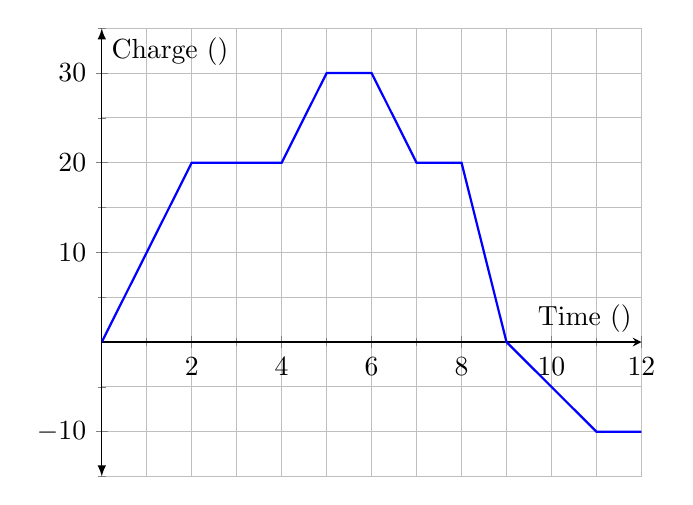
\begin{tikzpicture}[
		declare function={
			func(\x) = (\x < 2) * (10*\x)
			+ and(\x >= 2, \x < 4) * (20)
			+ and(\x >= 4, \x < 5) * (10*\x-20)
			+ and(\x >= 5, \x < 6) * (30)
			+ and(\x >= 6, \x < 7) * (-10*\x+90)
			+ and(\x >= 7, \x < 8) * (20)
			+ and(\x >= 8, \x < 9) * (-20*\x+180)
			+ and(\x >= 9, \x < 11) * (-5*\x+45)
			+ (\x >= 11) * (-10)
			;
		}
	]\label{fig:Q3ChargeTime}
    \begin{axis}[	xmin=0, ymin=-15, xmax=12, ymax=35,
    				xlabel={Time (\si{\second})}, ylabel={Charge (\si{\coulomb})},
    				legend pos=north west, 
    				domain=0:12,
    				grid=both,
    				axis lines=middle,
    				minor tick num=1,
    				y axis line style={latex-latex}]
        \addplot[blue, thick] {func(x)};

        %\legend{$3(x-2)^2$}
    \end{axis}
	\end{tikzpicture}
\end{center}
\fi

\begin{solutionorgrid}[10cm]
	\begin{center}
	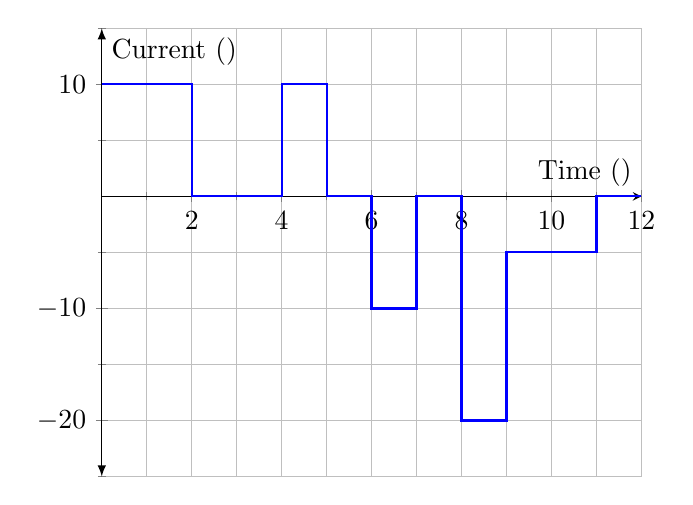
\begin{tikzpicture}\label{fig:Q3CurrentTime}
    \begin{axis}[	xmin=0, ymin=-25, xmax=12, ymax=15,
    				xlabel={Time (\si{\second})}, ylabel={Current (\si{\ampere})},
    				legend pos=north west, 
    				domain=0:12,
    				grid=both,
    				axis lines=middle,
    				minor tick num=1,
    				y axis line style={latex-latex}]
        \addplot+[blue, thick, mark=none,const plot]
		coordinates
		{(0,10) (2,10) (2,0) (4,0) (4,10) (5,10) (5,0) (6,0) (6,-10) (7, -10) (7, 0) (8, 0) (8, -20) (9, -20) (9,-5) (11, -5) (11, 0) (12, 0)};
    \end{axis}
	\end{tikzpicture}
\end{center}
\end{solutionorgrid}

\question Given:
\begin{equation*}
	v(t) = 4\sin(3t+4)
\end{equation*}
\begin{parts}
	\part Determine the amplitude of the voltage.
	
\end{parts}

\end{questions}